%This file will contain our design approach
%Describe the basis and then the architecture here - for example how do you calculate medians, what kind of parallelism model is employed? How often do you need to synchronize? etc.
\subsection{Query 1}
In the context of query 1, time is divided into multiple slots of different time slice sizes. The time slice sizes considered are 1m, 5m, 15m, 60m \& 120m. Hence for a day we have twelve 120m slices and 86400 one minute slices. When processing the events falling withing a time slice, Query 1 should output predicted load of each plug and the house for the next to next time slice. Query 1 should output the load prediction based on the average load of current time slice and the median of the historical load averages of the future time slice for which we are making prediction. We need to produce forecast every 30s.

We have one house process for each house in the data set and a broker process. The broker process reads the data from the input stream (sorted events file in current implementation) and passes it to the corresponding house process. Communication between the processes is done via operating system sockets.

In the house process, we have load value accumulators for different time slices (1m, 5m, 15m, 60m & 120m). We also have another accumulator for 30s. When house process gets an event if the event falls within the current 30s time slice, the load\footnone{For now we are ignoring events with work values.} value is added to the 30s accumulator & the count of values is incremented. If the event crosses the 30s timeslice, then the accumulated load values and count is added to accumulators of all the other time slices (1m, 5m.. etc) and a forecast output is triggered, before setting the 30s accumulator to current load value and count to 1. The triggered forecasting will output the predictions for all the time slices with the average of current accumulated load values and the historical median of the corresponding future time slice. The accumulators for each time slice gets reset, if we get an event crossing the time slice boundary, after making the forecast using the accumulater load value.


\subsubsection{The Median Algorithm for query 1}
For this query, to forecast the load of a plug in a time slice of a specific size, we need the median of the previous average loads for that time slice and for that slice size. For each day and each plug, we have only one value per day of data for that time slice and slice size. So, we store all these values in a container.

In the median container we maintain two heaps. Out of the two, one is a min-heap and the other is a max-heap. Each heap contains about half of the values. Now following three cases can occur:
\begin{itemize}
\item Case 1: The min-heap contains one more element than the max-heap. In this case, the median is the topmost value of min-heap.
\item Case 2: The max-heap contains one more element than the min-heap. In this case, the median is the topmost value of max-heap.
\item Case 3: Both the min-heap and the max-heap contain equal number of elements. In this case, the median is the average of the topmost value of min-heap and the topmost value of max-heap.

\end{itemize}

\section{Query 2}
The goal of query 2 is to identify outliers that consume significantly higher amount of energy compared with the average consumption computed globally. A plug is counted as an outlier if median load of the plug is more than the median load of all the plugs in the system for a given sliding window (1 hr or 24 hrs). We need to produce an output event when the percentage of such plugs in a house changes from the previous position of the sliding window. 

\subsection{Architecture}
To evaluate Query 2, we have to compute global median i.e. median of all the data of all the plugs in the system acquired in a given sliding window of length 1 hr and 24 hrs. We compare the global median with the local plug medians and figure out the outliers in the system. All of this computation needs to be done every time we receive a new event. The frequent comparison of locally computed data with global data enforces a single node solution for all the houses in case of Query 2.

There are two processes in the system residing on different nodes. The broker process reads data from a file and sends events to the Q2 process. Q2 keeps a linked list of all the events of last 24 hrs in the order they have been received. Whenever a new event is received by Q2, we slide the window such that some of the events from the tail of the linked list are removed and the new event is inserted at the head. Further, required plug medians and global median are recomputed and change in the number of outlier plugs is written to the output file (denoting an output event).

\begin{figure}[h]
\begin{center}
\begin{tikzpicture}[scale=0.7, >=stealth', transform shape, shorten >=1pt, node distance=4cm,auto]
\tikzstyle{every state}=[draw=blue!50, very thick, fill=blue!20,minimum size=2cm]
\node[state] (broker) [text width=1.5cm, align=center] {Broker Process};
\node[state] (Q2) [right of=broker] {Q2 Process};

\path[->] (broker) edge node {events} (Q2);
\end{tikzpicture}
\caption{System Architecture (Query 2)}
\end{center}
\end{figure}
\vspace*{-0.3cm}

We use the Sliding Median Container (SlidingMc) in order to compute various medians and S Container (SCont) for the purpose of finding the number of outliers in every house. Let's assume an event \textit{E} is received by the Q2 process from the broker process with timestamp \textit{$T_E$}. Let's also assume the window size to be \textit{W} seconds which can be either 1 hr or 24 hrs. \textit{$T_W$} is the minimum timestamp which exists in the window of length \textit{W} terminating with the event E as shown in the Figure \ref{fig:linked_list}.

\begin{figure}[h]
\begin{center}
\begin{tikzpicture}[scale=0.8, transform shape, shorten >=1pt, node distance=0.8cm,auto]
\tikzstyle{every state}=[draw=blue!50, rectangle, very thick, fill=blue!20]
\node[state] (I1) {$T_0$};
\node[state] (I2) [right of=I1] {};
\node[state] (I3) [right of=I2] {};
\node[state] (I4) [right of=I3] {$$};
\node[state] (I5) [right of=I4] {$T_W$};
\node[state] (I6) [right of=I5] {$$};
\node[state] (I7) [right of=I6] {$$};
\node[state] (I8) [right of=I7] {$$};
\node[state] (I9) [right of=I8] {$T_E$};

\draw [decorate,decoration={brace,amplitude=10pt,mirror,raise=10pt},yshift=0pt] (I5.center) -- (I9.center);
\node (text) at (5,-1) {Window W};
\end{tikzpicture}
\caption{Linked List in Q2 process \label{fig:linked_list}}
\end{center}
\end{figure}

Note that there may be multiple events with the timestamp $T_W$ in the window. In such a case, we choose the left most event with the same timestamp $T_W$ in the linked list. Also, if the data corresponding to the timestamp $\tau = (T_E - W +1)$ is missing, then $T_W$ will be the first timestamp bigger than $\tau$ for which event for any plug in the system is present. Now, the algorithm proceeds as follows. We shift the left end of the window one event, keeping the right end fixed. We delete the oldest event from the median container of the corresponding plug and the global median container. Now, we compute new median of the plug and insert the new median into the S container of the house. S container is, then, queried to find out whether the percentage of outliers for a given house has changed after the shift. We output an event if any of the percentage for any house has changed. On the other hand, if the global median doesn't change, we only check the percentage number of outliers for the house corresponding to the deleted event.

We stop when the leftmost event in the window has the timestamp $T_W$. In the last slide, before computing any medians, we also insert the newly received event $E$ into the global median container and the median container of the plug of the event E. Rest of the computation remains same. To avoid redundant storage of the data, we keep the linked list only for 24 hrs sliding window, and keep a pointer to the first event of the 1 hr window in the same linked list.


\subsection{Median Algorithm}
In query 2, we have to compute the median of large amounts of data frequently. A trade off exists between the computational complexity and accuracy of the median so derived. We define a container which provides the basic functionality of inserting a new element, deleting a given element and finally providing the approximate median for currently existing data in the container. We first insert all the elements into the container corresponding to the sliding window. Every time we slide by 1 sec, we perform at most 2 operations. We delete the oldest event if it exists and insert the latest event in the window. Every insert and/or delete operation is followed by computation of median. We, therefore, want to minimize the complexity of median calculation. We, now, propose an algorithm to compute median which takes constant time for every operation in the given scenario with very low relative error.

The basic idea is to construct a histogram of the data using fixed number of bins (M-1)\footnote{The Algorithm is inspired from discussions on \url{http://stackoverflow.com/questions/638030}} . The histogram is then queried to find median of the data. We sort the first M distinct values inserted into the container and use them in order to build up the (M-1) bins. Every $i^{th}$ inserted value corresponds to the starting of $i^{th}$ bin and every bin is associated with a frequency. Frequency denotes the frequency of the data greater than equal to $i^{th}$ lowest value (including) and less than $(i+1)^{th}$ lowest values (excluding) among M inserted value into the container. We also store the index of the bin containing the median after an insertion or deletion is performed, cumulative sum of the frequencies upto and including the bin in which median resides and the total number of values inserted into the container.

Every time a new value is inserted, the frequency of the corresponding bin is incremented. On the other hand, if a value is to be deleted, the frequency of the corresponding bin is decremented. At the time of insertion or deletion, we also modify the variable storing the index of the bin having the current median and accordingly the cumulative sum. The corresponding bin to insert/delete can be found in $\log(M)$ order complexity where (M-1) represents the number of bins. We handle below cases as follows-
\begin{itemize}
\item If frequency of a bin becomes significantly higher than some constant times the average bin frequency, we split the bin into two bins. Every new bin is given half of the frequency of the original bin. The range of values is also equally divided between 2 bins.
\item If frequency of a bin reaches to zero, we simply delete the bin.
\item If an inserted value is less than the lowest value or higher than the highest value present in the median container, we create another bin starting with the inserted value.
\item If number of bins are higher than the maximum allowed number of bins, we merge 2 bins. These 2 consecutive bins are chosen such that they have minimum total frequency than any other two consecutive bins. The frequency of the higher bin is added to the frequency of the lower bin and the higher bin is deleted.
\end{itemize}

We implemented median container using an array. Arrays provides the flexibility of binary search which is required to be done frequently in our case. We keep two empty memory slots on both sides of the array, which simplifies an insertion of a new bin in case of inserted value not being in the existing range of values. When a new bin is inserted/merged in the middle of the array, we shift the rest of the array to fill up the void.  We used low level operation \textit{memmove} provided by cstring library in C++, in order to speed up the shift operation.

In this case we need to compute the median every time we receive an event. So every insert or deletion or both will be followed by a call to the \textit{getMedian} function of the container.  We modify the variable storing the index to the bin having the current median, at the time of insert and delete only.

\begin{table}[h]
\begin{center}
\begin{tabular}{|c|c|c|}
\hline 
 & \textbf{Worst Case} & \textbf{Average Case} \\ 
\hline 
\textbf{insert} & O(M) & O($\log(M)$) \\
\hline 
\textbf{delete} & O(M) & O($\log(M)$) \\
\hline 
\textbf{getMedian} & O(1) & O(1) \\ 
\hline 
\end{tabular} 
\end{center}
\end{table}

\subsection{Relative Error for Median Container}
In this case, we did 1000 experiments, each inserting 50000 random values into the container. The CDF is plotted in the Figure \ref{fig:relative_error}. It can be observed that there is very low relative error due to the approximation. 

\begin{figure}[h]
\begin{center}
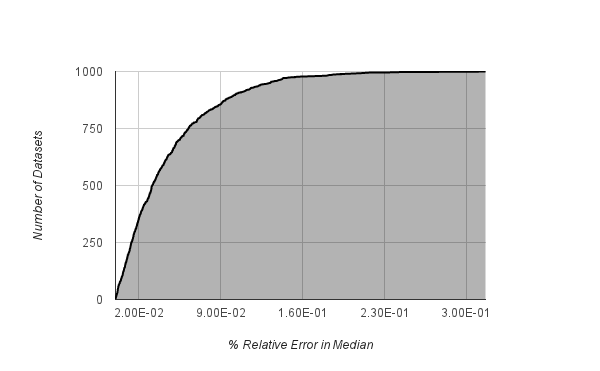
\includegraphics[scale=0.5]{img/relative_error}
\caption{CDF of Relative Error \label{fig:relative_error}}
\end{center}
\end{figure}

\subsection{Choosing the Number of Bins}
We did several experiments with the median container in order to figure out an optimum number of bins. The Number of bins affects the accuracy of the computed median. We used ten datasets generated randomly with different mean and variance. We used different number of bins ranging from 100 to 2000 for each dataset and calculated relative error in each case.

\begin{figure}[h]
\begin{center}
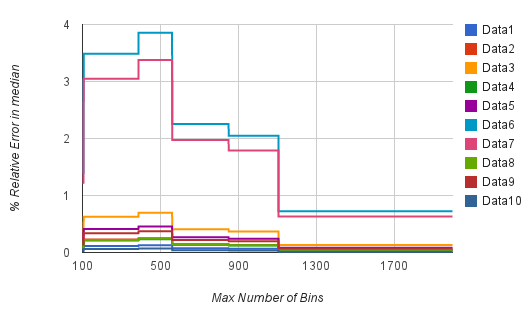
\includegraphics[scale=0.5]{img/bin_size_experiment}
\vspace*{-0.4cm}
\caption{\% Relative Error vs No of Bins \label{fig:binsize}}
\end{center}
\end{figure}

As evident from Figure \ref{fig:binsize}, bin size greater than 1200 gives the lowest error. We used bin size equal to 1200 while running Query 2.

\subsection{S Container}
We have to compute the number of plugs in a house having higher median load than the global median load (median load of all the plugs in the system). In order to efficiently compute this, we defined another container termed the $S$ container. The $S$ container stores median values of all the plugs in a house and evaluates the number of plugs higher than the global median. It provides basic operation of inserting (replacing) a newly computed plug median for the house, and finding out number of plugs which have higher median load than the global median (getNumOfLargeNum).

The issue here is, that we don't know number of plugs in a house before hand. It has to be acquired as the system makes progress. Hence, we had to use a map (key-value storage) in order to store the data but that leads to O(K) complexity of the \textit{getNumOfLargeNum} operation where K is the total number of plugs in a house. We avoided this by again using an array and stored all the data in sorted order with key being the plug median. When a new value is to be inserted, we require the old plug median in order to search the location of the plug data in the array. As soon as we find the location, we replace the new median with the old median and modify the location such that the array is sorted again.

The asymptotic complexity of this is also O(K) but in the given scenario, a momentous change in median values are unlikely. It will take finite number of more than one steps which will lead to significant change in the median values. In such a case, very little movement will be required while sorting the array after an insertion is performed. On the other hand, \textit{getNumOfLargeNum} operation will always be $\log(K)$.

%We do not store the whole measurement (16 byte) in the array but just the pointers (4 byte) to those measurements, which leads to even less amount of shift in the data. We use \textit{memmove} operation provided by CString library of C++, rather than manual copying of the array to increase the performance of the container.

%\subsection{Linked List Window}
 
\subsection{Experimental Evaluation}
We use the same setup as we used in case of Query 1. The broker process is executed on 1 Virtual Machine and Q2 process is execute on another virtual machine in the same cluster. We are able to achieve a constant average throughput of 480 thousand events per sec as shown in Figure \ref{fig:q2_throughput}

\begin{figure}[h]
\begin{center}
	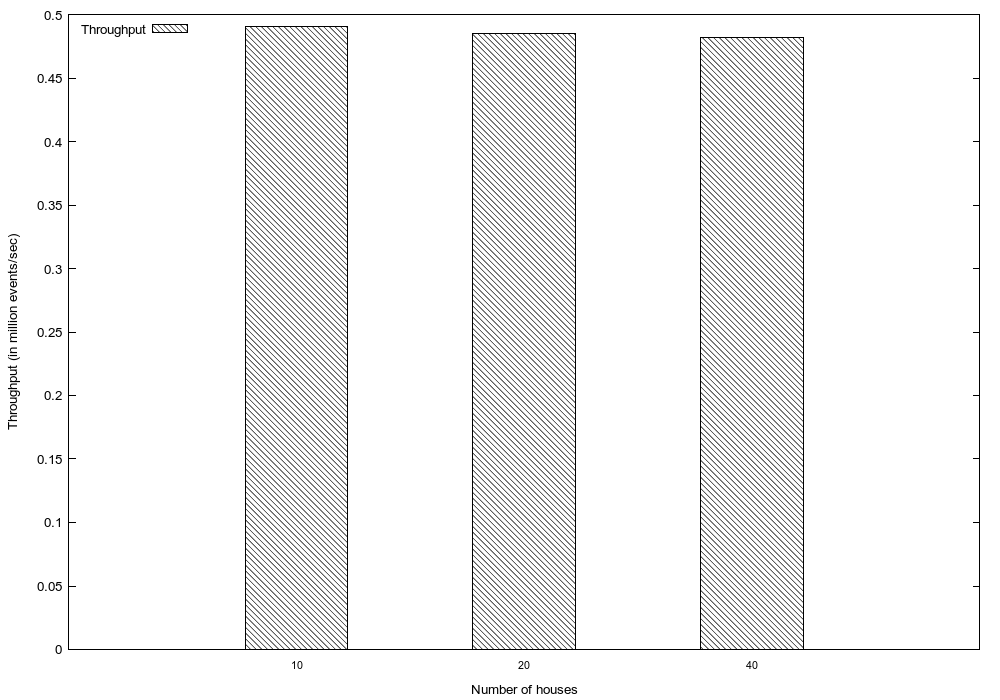
\includegraphics[scale=0.55]{img/q2_throughput}
	\vspace*{-0.4cm}
	\caption{Throughput vs No. of Houses (Query 2) \label{fig:q2_throughput}}
\end{center}
\end{figure}

\vspace*{-0.5cm}
Because there is only one Q2 process computing all the percentage values, throughput doesn't change significantly in terms of events/sec as the number of house increases. The utilization level in case of Q2 process is always close to 100\% as shown in Figure \ref{fig:q2_util}.

\begin{figure}[h]
\begin{center}
	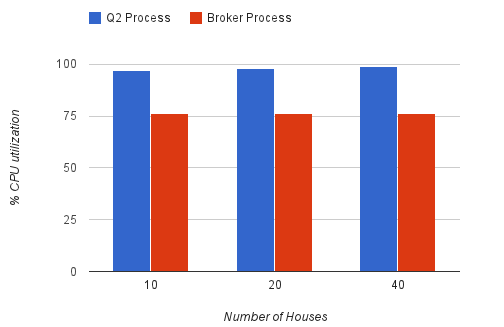
\includegraphics[scale=0.55]{img/q2_utilization}
	\vspace*{-0.3cm}
	\caption{\% Util vs No. of Houses (Query 2) \label{fig:q2_util}}
\end{center}
\end{figure}

\vspace*{-0.4cm}

\begin{figure}[h]
\begin{center}
	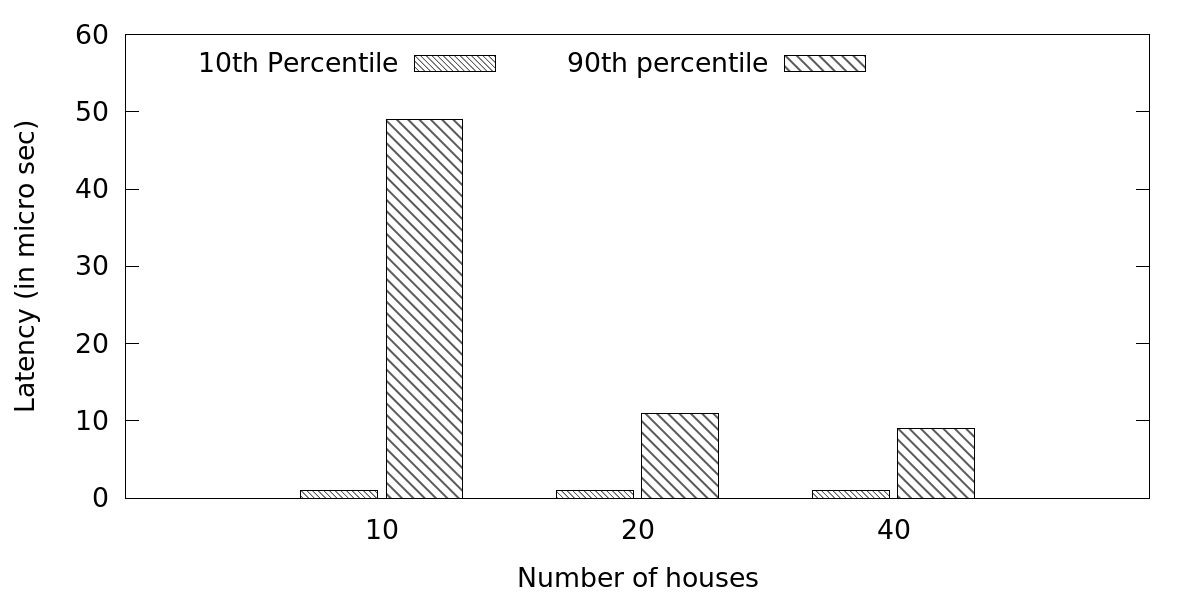
\includegraphics[scale=0.6]{img/q2_latency}
	\vspace*{-0.3cm}
	\caption{Latency vs No. of Houses (Query 2) \label{fig:q2_latency}}
\end{center}
\end{figure}

\vspace*{-0.4cm}
Latency corresponding to an output event, in case of Query 2, is defined as the amount of time taken to output event after the corresponding input event is received. Note that one input event may result in more than one output events and latency of the events output later will be higher. Latency graph for Query 2 is shown in Figure \ref{fig:q2_latency}. 90\% for 10 houses is higher because of biased distribution of data with respect to house. Houses 0-9 have more amount of data and the number of output events, therefore, will be more for every input event. In such a case, the events output later will have higher latency values.
